\documentclass{article}
\usepackage[margin=.75in]{geometry}
\usepackage{amsthm, amsmath, amssymb, amsfonts}
\usepackage{graphicx}
\usepackage[backend=bibtex8]{biblatex}

\bibliography{BioInfCite}


\begin{document}
\begin{enumerate}
	\item 
	\begin{enumerate}
		\item[(1)] Scoring scheme 5. A perfect alignment would be all matches. A match should grant more points than anything else. This is the only scheme that does this.
		\item[(2)] Scoring scheme 4. This could be somewhat reasonable if the only goal was to identify sequences of the same length.
		\item[(3)] Scoring scheme 1. This should align the sequences as far apart as possible, but where they meet should be as much matches as possible. Doesn't make sense, but it's better than the others.
		\item[(4)] Scoring scheme 3. Same as scheme 1, but more points for further apart sequences.
		\item[(5)] Scoring scheme 2. This will just try to make gaps. It doesn't care about anything else.
		\item[(6)] Scoring scheme 6. Avoid matches, prefer gaps. This makes no sense.
	\end{enumerate}
	\item 2 cases. The first is when there is no gap (or the gap is size 0, or it is to the left of the first or the right of the last base). In this case, there are 8 ways to place the bases on their row. The second case is when the gap is at least size 1 and between two bases. In the second case, there are 4 places to put the gap, and $8-g$ ways to place the sequence on the grid for a gap of size $g$. There are $8 + 4(7+6+5+4+3+2+1) = 120$ arrangements for each row, leading to a grand total of $120^6 = 2\,985\,984\,000\,000$ total possible grid arrangements. Some of these will be effectively the same alignments.
	\item RAGM $\rightarrow 4,4,4,1$ possible base pair sequences for each, respectively. Total would be $4\times 4\times 4\times 1 = 64$ possible DNA substrands.
	\item \begin{enumerate}
		\item 19 possible substitutes for any amino acid, with 5 choices of amino acid, is $19\times 5 = 95$ possible mutants.
		\item Same number of possible first mutations, times $19\times 4$ choices for the second mutation, for $95\times 19\times 4 = 7220$ possible mutations. Divide that by 2 because there is no difference based on which was chosen first, for $3610$ total possible mutations.
		\item 19 replacement choices for each amino acid mutated is $19^k$. `Order' the $n$ amino acids $n!$ different ways, select the first $k$, divide by the number of ways those could be ordered and divide by the number of ways those not selected could be ordered. $$19^k \frac{n!}{k!(n-k)!}$$
	\end{enumerate}
\end{enumerate}
\pagebreak
\section*{Introduction \& Motivation}
The goal of this paper is to explore the effects of \textit{splicex} on the wild type of the protein best fitting a certain protein sequence. The protein sequence was found to best match Barnase. The purpose of the drug is to disrupt the function of the protein through mutating a Phenylalanine in the wild type protein to either an Alanine or a Lysine.
\section*{Methods}
First I used protein BLAST \cite{BLAST} to try to identify the protein, which matched very well to Barnase and many of its mutants. Unfortunately, the PDB entry for Barnase was not included in the BLAST result, so I had to perform a PDB search and use my best judgment to determine the wild type protein entry. Because there multiple entries, I decided to incorporate the results from two difference PDB entries into my results, each referring to wild type Barnase. From here I simply used SDM (Site Directed Mutator) \cite{SDM} to predict change in stability ($\Delta\Delta G$) for each mutation. I additionally cross referenced the results with a Barnase PDB entry that represented wild type Barnase interacting with a ligand, as that would provide insight into Barnase while functioning.
\section*{Swap Rankings}
\begin{tabular}{|l l|r|r|r|}
\hline
Residue & Mutation & 1BNR & 1BNS & 1A2P\\\hline
82 & Alanine & +0.78 &  +0.78 & +0.78 \\\hline
7 & Lysine & +0.23 & +0.26 & +0.14 \\\hline
82 & Lysine & -0.02 & -0.14 & -0.14 \\\hline
7 & Alanine & -2.08 & -0.34 & +0.97 \\\hline
56 & Lysine & -1.50 & -0.07 & -0.27 \\\hline
56 & Alanine & -3.79 & -1.55 & -0.60 \\\hline
106 & Lysine & -1.51 & -1.53 & -1.50 \\\hline
106 & Alanine & -3.80 & -3.80 & -3.73 \\\hline
\end{tabular}
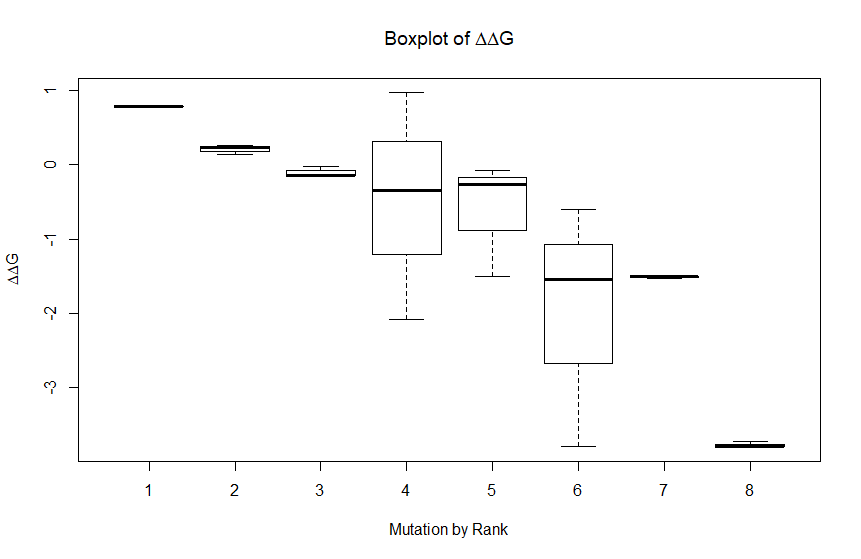
\includegraphics[width=.55\textwidth]{DeltaDeltaGBoxplot.png}
\section*{Justification}
\begin{enumerate}
	\item 82A has consistent structural disruption. Clear winner.
	\item 7K has little structural disruption.
	\item 82K simply has nearly 0 effect, but consistently negative.
	\item 7A is high variance. It's difficult to determine what the true effect of this mutation most likely is, so I rank it poorly. Minimizing my chance of a false positive ranking.
	\item 56K is relatively near 0, but is high variance.
	\item 56A is inconsistent, so while it does have very low $\Delta \Delta G$, there is better chance the prediction is off compared to lower ranked predictions.
	\item 106K is consistently stabilizing. Seems mutating residue 106 is unlikely to disrupt the protein.
	\item 106A is clearly predicted to stabilize the protein. All samples contain very significant negative $\Delta\Delta G$ scores.
\end{enumerate}
\section*{Conclusions}
Phenylalanines 7 and 82 seem to have the most significant impact on the protein's structure, with mutations in those positions predictively causing the most disruption when mutated. I conclude the most likely choice for \textit{splicex} to disrupt the protein is to replace the Phenylalanine at residue 82 with an Alanine.
\printbibliography
\end{document}